\subsection{Overview}

The second part of this project was focused on producing a library of HSL analogue-ciprofloxacin conjugates. The HSL head group was replaced with a selection of cyclic amines found in known quorum sensing modulators (see \ref{sec:AIA_intro}). 
The analogues were linked to ciprofloxacin \compound{cmpd:Cip} in two ways: directly using either an S$_N$2 reaction or peptide coupling, and via the triazole linkage shown previously (see \ref{sec:Tris}).

\subsubsection{Head groups}

The head groups used in this study are shown in \ref{fig:head_groups}. The cyclohexanol derivatives were synthesised as a diastereomerically pure racemate, whereas the cyclopentanol derivatives were synthesised as separate enantiomers. 
Although the timescale of this project prevented the inclusion of the cyclopentanone derivatives, these could be included in future work.
The 2-methoxybenzene derivatives do not have precedents as quorum sensing modulators in the literature, but they were included so as to be compared with the 3-methoxybenzene derivatives.

\begin{figure}[H]
	\begin{center}
		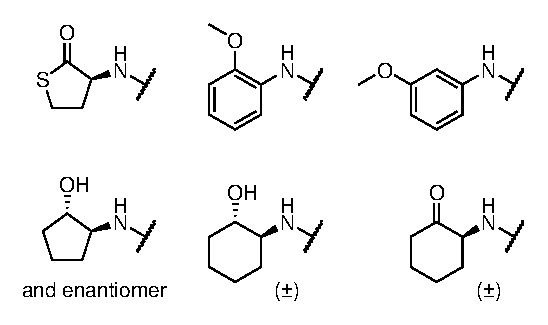
\includegraphics[scale=1]{head_groups}
		\caption{The head groups used in this section.\label{fig:head_groups}}
	\end{center}
\end{figure}

\subsubsection{Library construction}

As Ganguly \textit{et al.}\cite{Ganguly2011}  (see \ref{sec:AIA_intro}) synthesised their conjugate from Br-C$_4$-HCTL, it was envisaged that a branching strategy could be used to produce two sets of conjugates (see \ref{sch:branching_synth_general}). The first set would be formed by the S$_N$2 reaction of the relevant bromide with methyl ciprofloxacin. The second set would be made by displacing the bromide with azide, then performing a click reaction with the alkynyl ciprofloxacin derivative \compound{cmpd:Y4Cip} made previously to form the triazole-linked product. Cyclohexanone conjugates would be formed by oxidation of the alcohol conjugates.

\begin{scheme}[H]
	\begin{center}
		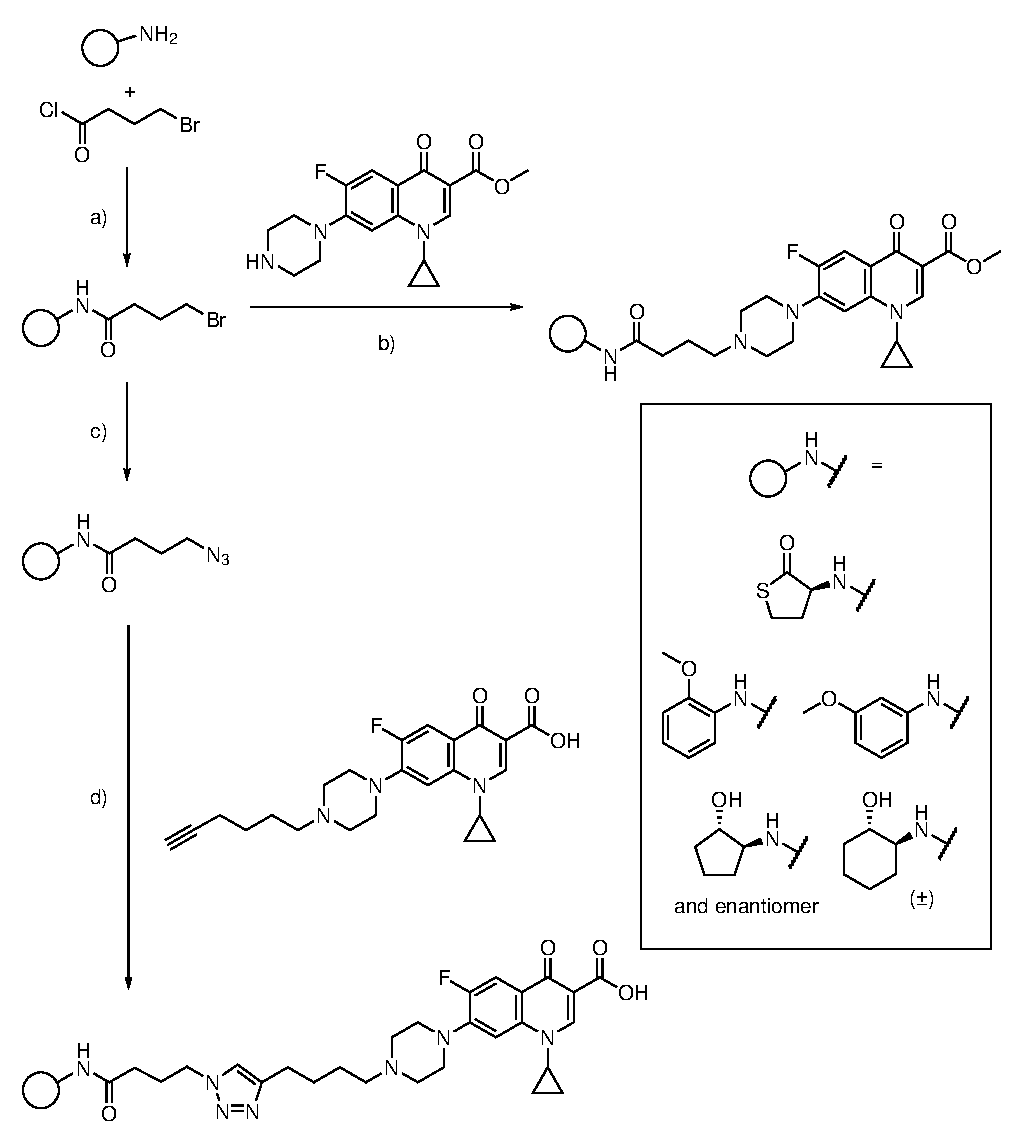
\includegraphics[scale=1]{branching_synth_general}
		\caption{General scheme showing the proposed branching synthesis of the HSL analogue-ciprofloxacin conjugates.\label{sch:branching_synth_general}}
	\end{center}
\end{scheme}

This strategy was successful for most head groups, but multiple side reactions were observed for the amino alcohol head groups and so other routes to these conjugates were investigated (see \ref{sec:HOcy5}).
